% This file is part of Mūlārthabodhinī XeLaTeX Source Code

% Mūlārthabodhinī XeLaTeX Source Code is free software: you can redistribute it and/or modify it under the terms of the GNU General Public License as published by the Free Software Foundation, either version 3 of the License, or (at your option) any later version.

% Mūlārthabodhinī XeLaTeX Source Code is distributed in the hope that it will be useful, but WITHOUT ANY WARRANTY; without even the implied warranty of MERCHANTABILITY or FITNESS FOR A PARTICULAR PURPOSE. See the GNU General Public License for more details.

% You should have received a copy of the GNU General Public License along with Mūlārthabodhinī XeLaTeX Source Code. If not, see <https://www.gnu.org/licenses/>.

\documentclass[12pt]{article}
\usepackage{calc}
\usepackage{ragged2e}
\newlength{\bookspine}
\newlength{\spinemargin}
\newlength{\coverwidth}
\newlength{\coverheight}
\newlength{\coverinside}
\newlength{\covermargin}
\newlength{\flapwidth}
\newlength{\coverbleed}
\newlength{\mylengthone}
\newlength{\mylengthtwo}
\newlength{\mylengththree}
\newlength{\mylengthfour}
\newlength{\ltwidth}
\newlength{\ltheight}
\newlength{\bkwidth}
\newlength{\bkheight}
\setlength{\coverwidth}{184mm} 
\setlength{\coverheight}{252mm} 
% http://www.askprint.co.uk/howto/Hardback-book-cover-specifications.php
\setlength{\bookspine}{20.76mm} 
\setlength{\spinemargin}{3mm} 
\setlength{\coverinside}{0mm}
\setlength{\covermargin}{15mm}
\setlength{\flapwidth}{50mm}
\setlength{\coverbleed}{3mm}
\setlength{\ltwidth}{\bookspine + \coverwidth*\real{2.0} + \coverinside*\real{2.0} + \flapwidth*\real{2.0}}
\setlength{\ltheight}{\coverheight + \coverinside*\real{2.0}}
\setlength{\bkwidth}{\ltwidth + \coverbleed*\real{2.0}}
\setlength{\bkheight}{\ltheight + \coverbleed*\real{2.0}}
\usepackage[dvips=false,pdftex=false,vtex=false,margin=0in,paperwidth=\ltwidth,paperheight=\ltheight]{geometry}
\usepackage[noaxes,noinfo,cam,dvips,pdftex,center,width=\the\bkwidth,height=\the\bkheight]{crop}
\usepackage[dvipsnames,prologue,table]{pstricks}
\usepackage{pst-all}
\usepackage{pst-text}
\usepackage{wallpaper}
\definecolor{Hanuman}{rgb}{0.9568627,0.4313725,0.1686275}
\usepackage{graphicx}
\usepackage{rotating}
\usepackage{xcolor}
\usepackage[ISBN=978-93-82253-06-8]{ean13isbn}
\usepackage{polyglossia}
\usepackage{relsize}
\setmainlanguage{hindi}
\setotherlanguage{english}

\setmainfont[Script=Devanagari, Path = ./, Extension = .ttf,UprightFont = *-Regular, BoldItalicFont = *-BoldItalic, BoldFont = *-Bold, ItalicFont = *-Italic, Mapping=devanagaridigits]{ChanakyaSanskrit}
\newfontfamily\engtextfont[Path = ./, Extension = .ttf,UprightFont = *R, BoldItalicFont = *BI, BoldFont = *B, ItalicFont = *I]{CharisSIL}
\newfontfamily\unifont[Path = ./, Extension = .ttf,AutoFakeBold=2.0]{arialunicodems}
\newfontfamily\rupeefonttwo[Path = ./, Extension = .ttf,]{Rupee_Foradian}

%\EANisbn[SC4]
\usepackage{hyperref}
\hypersetup{
	pdfstartview={XYZ null null 1},
	bookmarks=false
}
\setlength{\parindent}{0pt}
\begin{document}
\pagecolor{Hanuman}
\pagestyle{empty}
\psset{unit=1in}
\begin{pspicture}(\ltwidth,\ltheight)

% Draw the guides here
% 1. The layout
%\psframe[linecolor=white](0,0)(\ltwidth,\ltheight)
% 2. The hardcover
\setlength{\mylengthone}{\ltwidth - \coverinside - \flapwidth} 
\setlength{\mylengthtwo}{\ltheight - \coverinside} 
\setlength{\mylengththree}{\coverinside + \flapwidth} 
%\psframe[linecolor=white](\flapwidth,\coverinside)(\mylengthone,\mylengthtwo)
% 3. The spine
\setlength{\mylengthone}{\flapwidth + \coverinside + \coverwidth} 
\setlength{\mylengthtwo}{\flapwidth + \coverinside + \coverwidth + \bookspine} 
\setlength{\mylengththree}{\coverinside + \coverheight} 
%\psframe[linecolor=white](\mylengthone,\coverinside)(\mylengthtwo,\mylengththree)

% 4. The printable area on backcover
\setlength{\mylengthone}{\flapwidth + \coverinside + \covermargin} 
\setlength{\mylengthtwo}{\flapwidth + \coverinside + \coverwidth - \covermargin} 
\setlength{\mylengththree}{\coverinside + \coverheight - \covermargin} 
\setlength{\mylengthfour}{\coverinside + \covermargin} 
%\psframe[linecolor=white](\mylengthone,\mylengthfour)(\mylengthtwo,\mylengththree)

% 4. The printable area on frontcover
\setlength{\mylengthone}{\flapwidth + \coverinside + \coverwidth + \bookspine + \covermargin} 
\setlength{\mylengthtwo}{\coverinside + \covermargin} 
\setlength{\mylengththree}{\ltwidth - \flapwidth - \coverinside - \covermargin} 
\setlength{\mylengthfour}{\coverinside + \coverheight - \covermargin} %\psframe[linecolor=white](\mylengthone,\mylengthtwo)(\mylengththree,\mylengthfour)

% 5. The printable area on spine
\setlength{\mylengthone}{\flapwidth + \coverinside + \coverwidth + \spinemargin} 
\setlength{\mylengthtwo}{\coverinside + \covermargin} 
\setlength{\mylengththree}{\flapwidth + \coverinside + \coverwidth + \bookspine - \spinemargin} 
\setlength{\mylengthfour}{\coverinside + \coverheight - \covermargin}
%\psframe[linecolor=white](\mylengthone,\mylengthtwo)(\mylengththree,\mylengthfour)

%%%%%%%%%%%%%%%%%%%%%%%%%%%%%%%%%%%%%%%%%%%%%%%%%%
% THIS IS THE BOOK FRONTCOVER
%%%%%%%%%%%%%%%%%%%%%%%%%%%%%%%%%%%%%%%%%%%%%%%%%%
\setlength{\mylengthone}{\flapwidth + \coverinside + \coverwidth + \bookspine} 
\rput[lb](\mylengthone,217.5mm){\parbox{\coverwidth}{\centering\fontsize{26}{39}\selectfont\color{white}{\textbf{गोस्वामी नारायणदास नाभाजी विरचित}}}}
\rput[lb](\mylengthone,203.5mm){\parbox{\coverwidth}{\centering\fontsize{40}{60}\selectfont\color{white}{\textbf{श्रीभक्तमाल}}}}
\rput[lb](\mylengthone,189.5mm){\parbox{\coverwidth}{\centering\fontsize{28}{42}\selectfont\color{white}{\textbf{(मूलार्थबोधिनी टीका सहित)}}}}
\newsavebox\IBox
\setlength{\mylengthone}{\flapwidth +\coverinside + \coverwidth + \bookspine + \coverwidth*\real{0.5} - 57.5mm}
\sbox\IBox{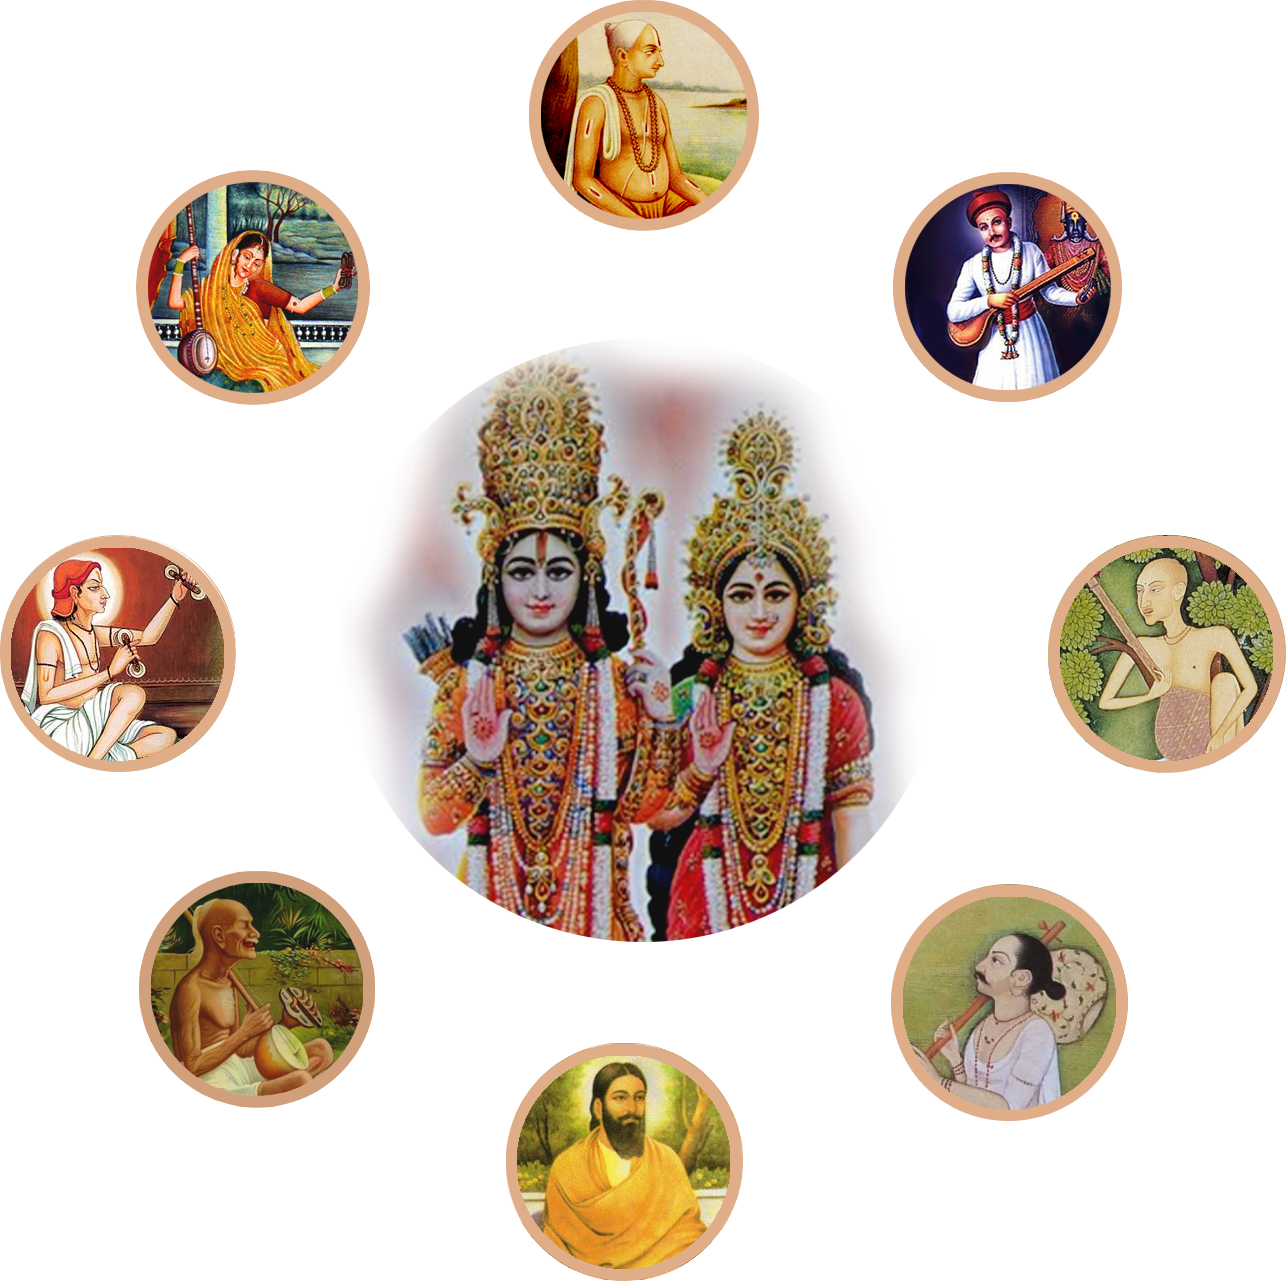
\includegraphics[width=115mm]{Bhaktamala2.png}}
\rput[lb](\mylengthone,62.5mm){\usebox\IBox}
\setlength{\mylengthone}{\flapwidth + \coverinside + \coverwidth + \bookspine} 
\rput[lb](\mylengthone,42.5mm){\parbox{\coverwidth}{\centering\fontsize{22}{33}\selectfont\color{white}{\textbf{टीकाकार}}}}
\rput[lb](\mylengthone,29.5mm){\parbox{\coverwidth}{\centering\fontsize{26}{39}\selectfont\color{white}{\textbf{जगद्गुरु रामानन्दाचार्य स्वामी रामभद्राचार्य}}}}

%%%%%%%%%%%%%%%%%%%%%%%%%%%%%%%%%%%%%%%%%%%%%%%%%%
% THIS IS THE BOOK SPINE
%%%%%%%%%%%%%%%%%%%%%%%%%%%%%%%%%%%%%%%%%%%%%%%%%%
%Book title on the spine
\setlength{\mylengthone}{\flapwidth + \coverinside + \coverwidth + \bookspine*\real{0.5} - 0.05mm} 
\rput[t](\mylengthone,225mm)
{\begin{turn} {-90}
	{\fontsize{22}{24.75}\selectfont\color{white}{\textbf{श्रीभक्तमाल (मूलार्थबोधिनी टीका सहित)}}}
\end{turn}}

% Author name on the spine
\setlength{\mylengthone}{\flapwidth + \coverinside + \coverwidth + \bookspine*\real{0.5} + 0.05mm} 
\rput[t](\mylengthone,87.5mm)
{\begin{turn} {-90}
	\fontsize{22}{24.75}\selectfont\color{white}{स्वामी रामभद्राचार्य}
\end{turn}}

% Publisher’s logo on the spine
\setlength{\mylengthone}{\flapwidth + \coverinside + \coverwidth + \bookspine*\real{0.5} - 0.05mm} 
\newsavebox\logobox
\sbox\logobox{
\includegraphics[width=16mm]{logo2.png}}
\rput[b](\mylengthone,15.25mm){\usebox\logobox}

%%%%%%%%%%%%%%%%%%%%%%%%%%%%%%%%%%%%%%%%%%%%%%%%%%
% THIS IS THE BOOK BACKCOVER
%%%%%%%%%%%%%%%%%%%%%%%%%%%%%%%%%%%%%%%%%%%%%%%%%%

\setlength{\mylengthone}{\flapwidth + \coverinside + \covermargin} 
\setlength{\mylengthtwo}{\coverwidth - \covermargin*\real{2}} 
\rput[tl](\mylengthone,230mm){\parbox{\mylengthtwo}{\fontsize{16}{20}\selectfont\color{white} 
\begin{sloppypar}\justifying\hyphenrules{nohyphenation} \textbf{मूलार्थबोधिनी} गोस्वामी नारायणदास नाभाजीकी अमर कृति \textbf{भक्तमाल}पर स्वामी रामभद्राचार्य द्वारा रचित हिन्दी टीका है। प्रस्तुत टीकामें भक्तमालके प्रत्येक पदके मूल अर्थको पौराणिक और लौकिक कथाओंके अनेक संदर्भों सहित विशद रूपसे समझाया गया है।\end{sloppypar}
\begin{sloppypar}\justifying\hyphenrules{nohyphenation} पद्मविभूषण जगद्गुरु रामानन्दाचार्य \textbf{स्वामी रामभद्राचार्य} भारतके प्रख्यात विद्वान्, शिक्षाविद्, बहुभाषाविद्, महाकवि, भाष्यकार, दार्शनिक, रचनाकार, संगीतकार, प्रवचनकार, कथाकार, व धर्मगुरु हैं। वे चित्रकूट-स्थित \textbf{श्रीतुलसीपीठ}के संस्थापक एवं अध्यक्ष और \textbf{जगद्गुरु रामभद्राचार्य दिव्याङ्ग विश्वविद्यालय}के संस्थापक एवं आजीवन कुलाधिपति हैं। स्वामी रामभद्राचार्य दो मासकी आयुसे प्रज्ञाचक्षु होते हुए भी २२~भाषाओंके ज्ञाता, अनेक भाषाओंमें आशुकवि, और शताधिक ग्रन्थोंके रचयिता हैं। उनकी रचनाओंमें चार महाकाव्य (दो संस्कृत और दो हिन्दीमें), रामचरितमानसपर हिन्दी टीका, अष्टाध्यायीपर गद्य और पद्यमें संस्कृत वृत्तियाँ, और प्रस्थानत्रयीपर (ब्रह्मसूत्र, भगवद्गीता, और प्रधान उपनिषदोंपर) संस्कृत और हिन्दी भाष्य प्रमुख हैं। वे तुलसीदासपर भारतके मूर्धन्य विशेषज्ञोंमें गिने जाते हैं और रामचरितमानसके एक प्रामाणिक संस्करणके संपादक हैं।\end{sloppypar}}}


% ISBN Barcode and logo
\rput[lb](176mm,38.75mm){\parbox{3cm}{\fontsize{11}{15}\selectfont\color{white}{\rupeefonttwo {\relscale{0.93} \textasciigrave}}\fontsize{10}{15}\selectfont\color{white}{\engtextfont 300}}}
\rput[rb](215mm,38.5mm){\parbox{0.75cm}{\fontsize{11}{15}\selectfont\color{white}{\rupeefonttwo {\relscale{0.93} \textasciigrave}}\color{white}{\fontsize{14}{15.75}\selectfont ३००}}}
\rput[r](215mm,26.5mm){\colorbox{white}{\EANisbn[SC2]}}

% put the logo on the back cover
\setlength{\mylengthtwo}{\coverinside + \covermargin + 10mm} 
\newsavebox\logoboxcover
\sbox\logoboxcover{
\includegraphics[width=0.75in]{logo2.png}}
\rput[lb](\mylengthone,\mylengthtwo){\usebox\logoboxcover}
% Publisher information
\setlength{\mylengthtwo}{\coverinside + \covermargin + 5mm} 
\rput[lb](\mylengthone,\mylengthtwo){\parbox{14cm}{\fontsize{14}{15.75}\selectfont\color{white}{\textbf{\ \ ज.रा.दि.वि.}}}}
\setlength{\mylengthtwo}{\coverinside + \covermargin} 
\rput[lb](\mylengthone,\mylengthtwo){\parbox{14cm}{\fontsize{10}{15}\selectfont\color{white}{\engtextfont www.jrhu.com}}}

\end{pspicture}
\end{document}